% !TeX spellcheck = cs_CZ
%{\tikzset{external/prefix={tikz/FYZI/}}
% \tikzset{external/figure name/.add={ch47_}{}}
%=========================== Kapitola: Zvuk. Vlnová rovnice =======================================
\chapter{Zvuk. Vlnová rovnice}\label{fyz:IchapXLVII}
\minitoc
  \section{Vlny}\label{fyz:IchapXLVIIsecI}
  \section{Šíření zvuku}\label{fyz:IchapXLVIIsecII}
  \section{Vlnová rovnice}\label{fyz:IchapXLVIIsecIII}
  \section{Řešení vlnové rovnice}\label{fyz:IchapXLVIIsecIV}
  \section{Rychlost zvuku}\label{fyz:IchapXLVIIsecV}
  \section{Příklady a cvičení}\label{fyz:IchapXLVIIsecVI}

    \begin{figure}[ht!] %\ref{fyz_fig457}
      \centering
      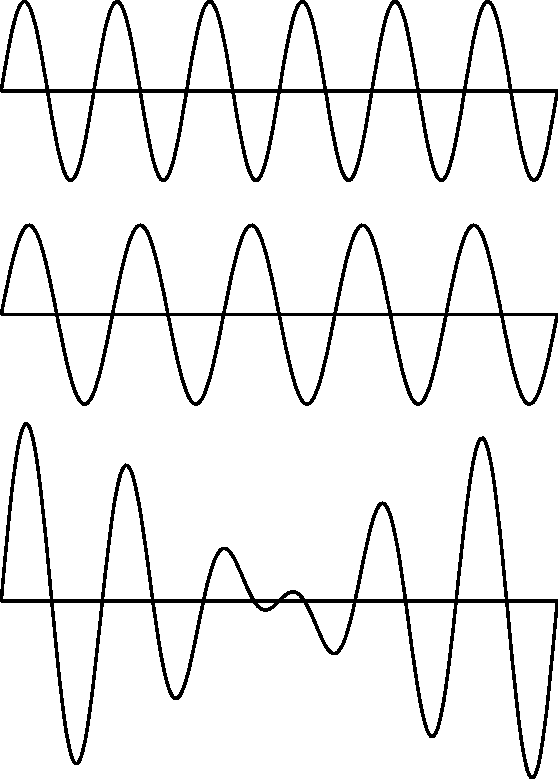
\includegraphics[width=0.7\linewidth]{fyz_fig457.pdf}
      \caption{ 
               (\cite[s.~707]{Feynman01})}
      \label{fyz_fig457}
    \end{figure}

    \begin{figure}[ht!] %\ref{fyz_fig458}
      \centering
      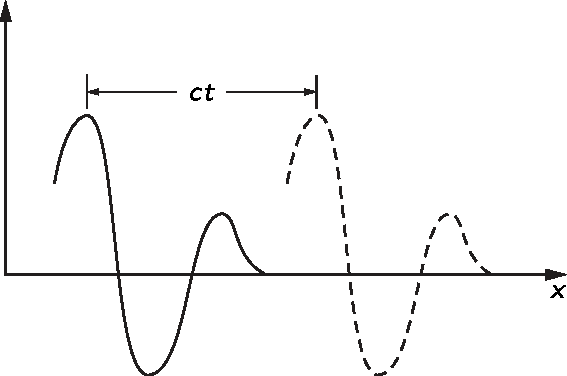
\includegraphics[width=0.7\linewidth]{fyz_fig458.pdf}
      \caption{ 
               (\cite[s.~707]{Feynman01})}
      \label{fyz_fig458}
    \end{figure}

    \begin{figure}[ht!] %\ref{fyz_fig459}
      \centering
      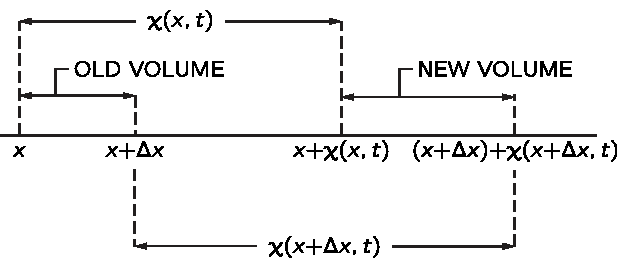
\includegraphics[width=0.7\linewidth]{fyz_fig459.pdf}
      \caption{ 
               (\cite[s.~707]{Feynman01})}
      \label{fyz_fig459}
    \end{figure}

    \begin{figure}[ht!] %\ref{fyz_fig460}
      \centering
      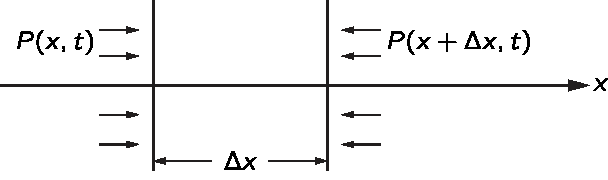
\includegraphics[width=0.7\linewidth]{fyz_fig460.pdf}
      \caption{ 
               (\cite[s.~707]{Feynman01})}
      \label{fyz_fig460}
    \end{figure}
    
%} %tikzset
%---------------------------------------------------------------------------------------------------
\printbibliography[title={Seznam literatury}, heading=subbibliography]
\addcontentsline{toc}{section}{Seznam literatury}